%\section{Hubo-Ach: Linux on Hubo}

\begin{figure*}[thpb]
  \centering
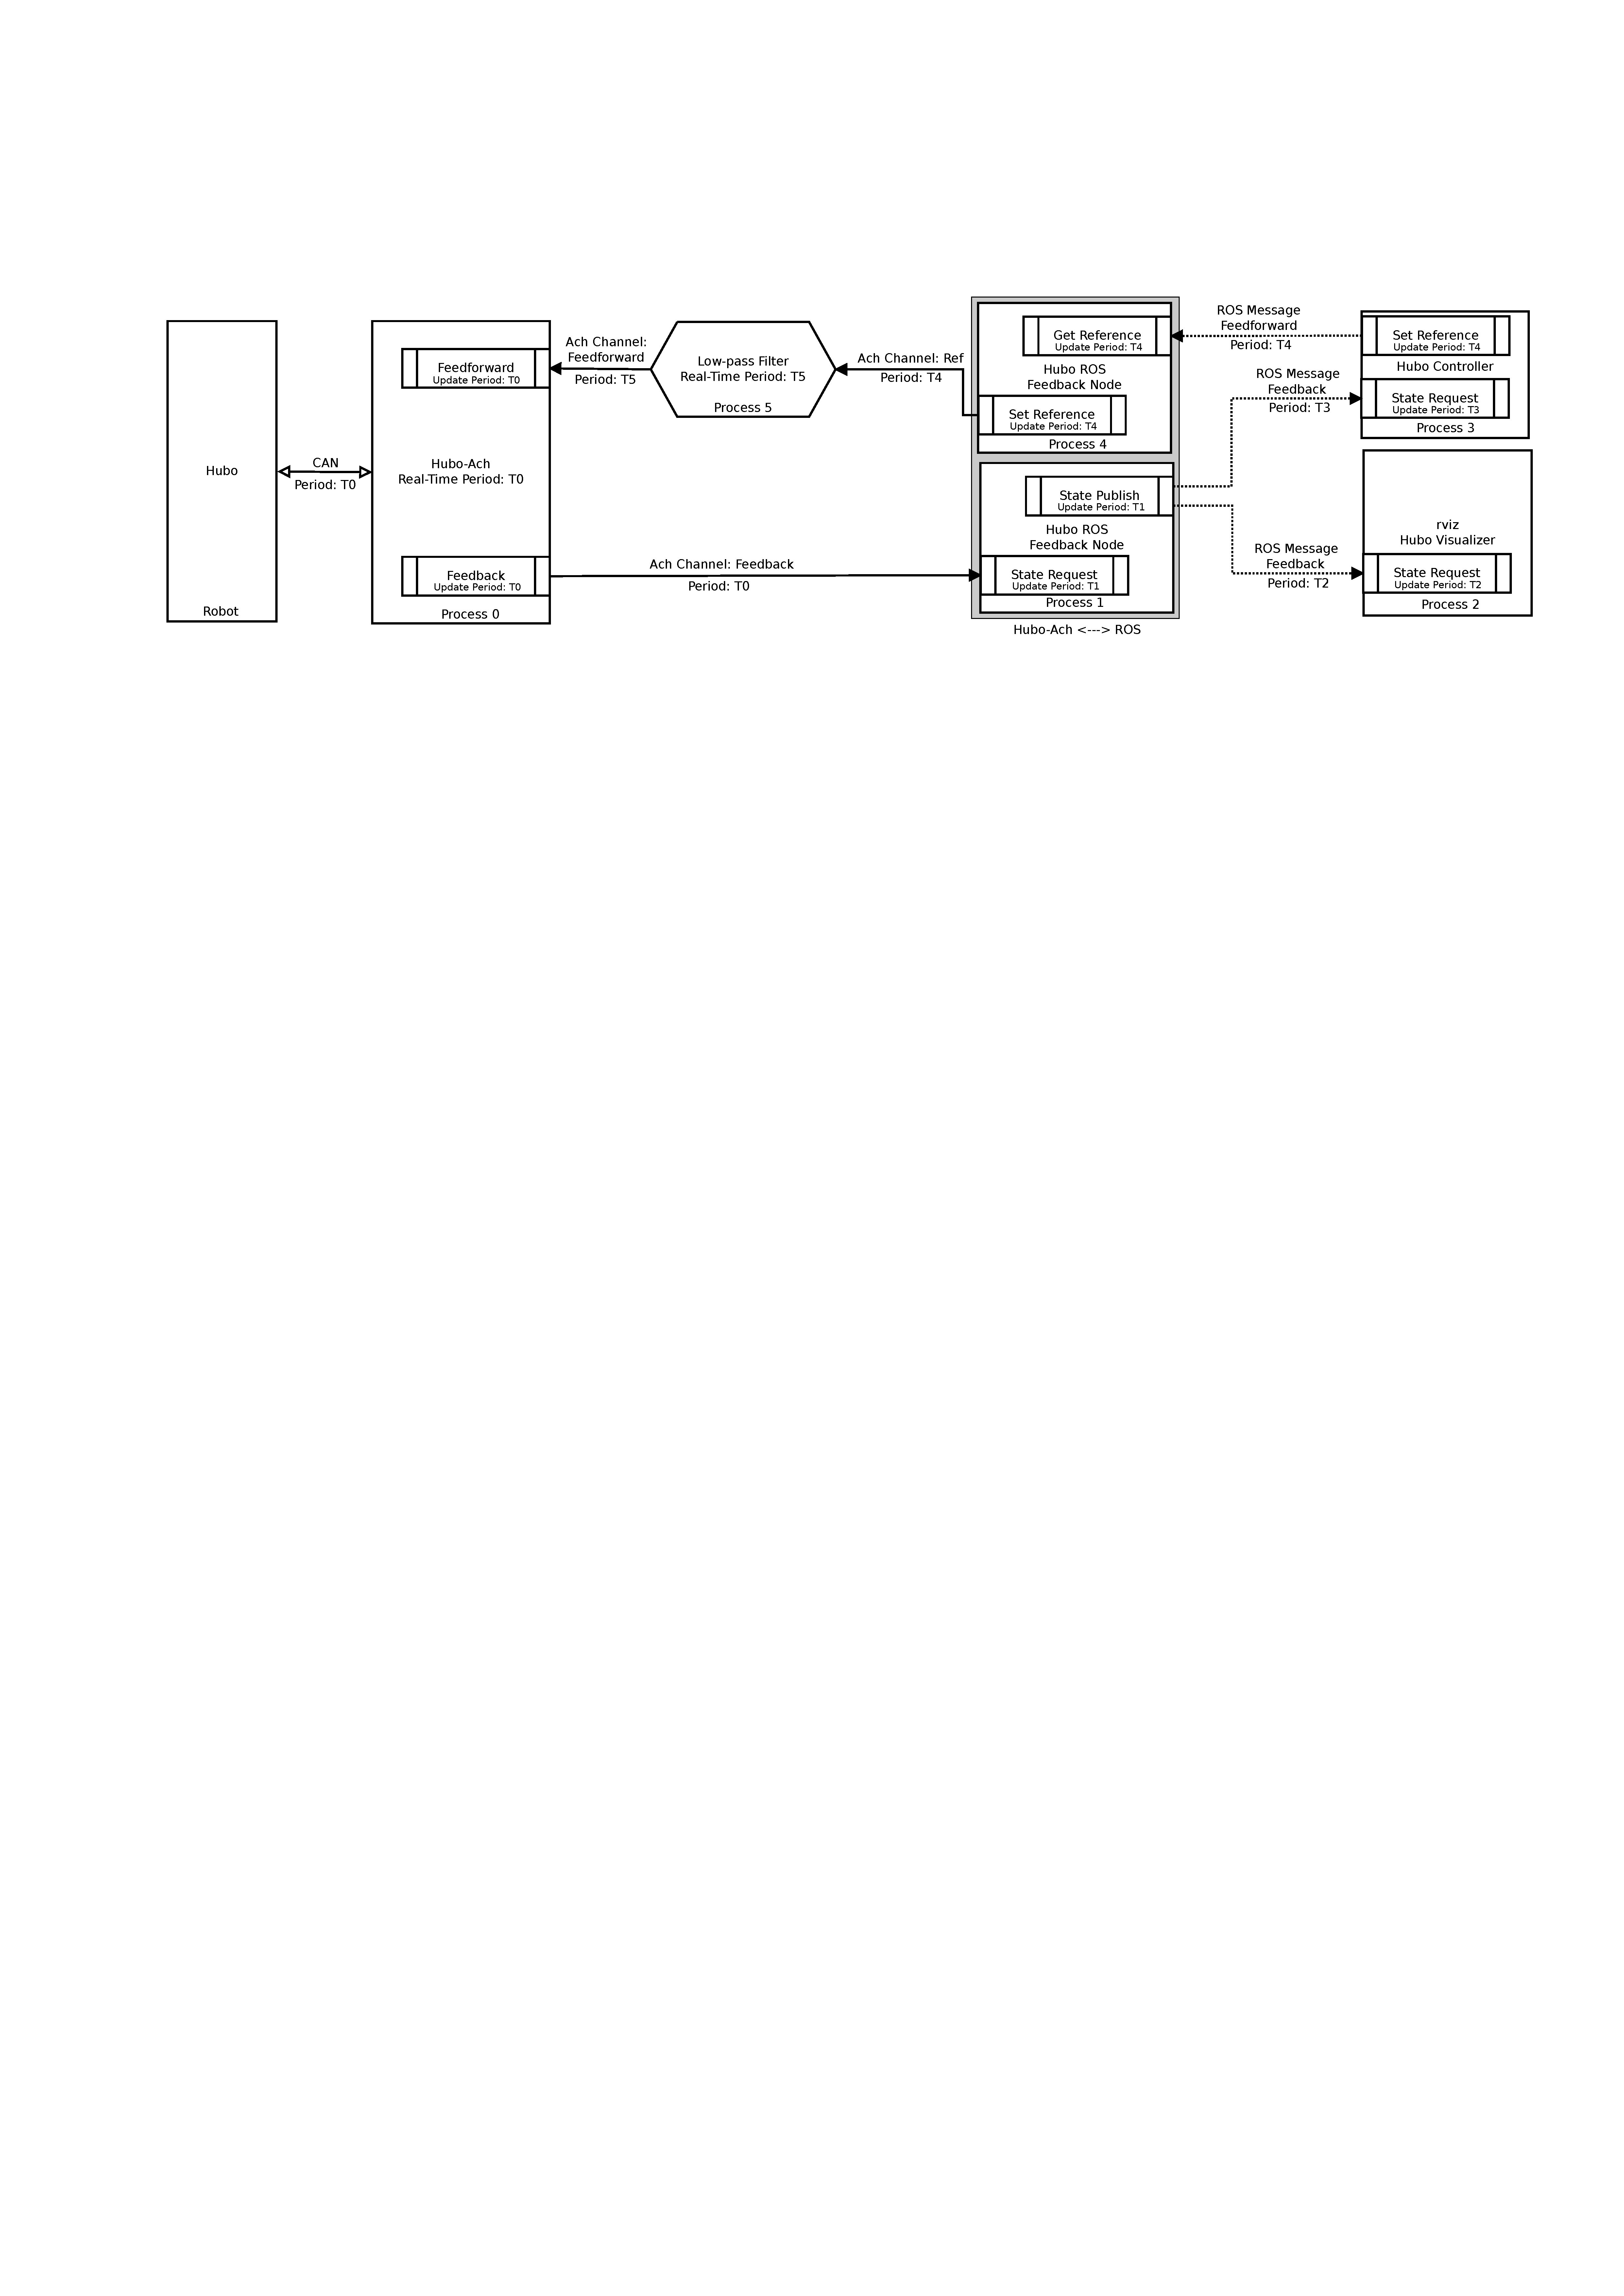
\includegraphics[width=2.0\columnwidth]{./pix/hubo-ach-diagram-ros.pdf}
  \caption{Hubo-Ach.}
  \label{fig:graph}
\end{figure*}


Hubo-Ach is the open-source, Linux based, BSD licensed control system run on Hubo.  
It was designed by Daniel M. Lofaro\footnote{Daniel M. Lofaro: http://danlofaro.com/} and Neil Dantam in collaboration with the \textit{Drexel Autonomous Systems Lab} at Drexel University and \textit{Golems - The Humanoid Robotics Laboratory}\footnote{Golems - The Humanoid Robotics Laboratory: www.golems.org/} at the Georgia Institute of Technology.  

The overarching goal of the Hubo-Ach system is to create an easy to use interface between the Hubo's electro-mechanical hardware and its programming environment.  
System design decisions were made with the programmers and developers of the Hubo in mind.
This design philosophy streamlines closed-loop controller implementation, human robot interaction development and the utilization of popular robot related systems such as ROS\footnote{ROS: http://www.ros.org/} (Robot Operating System), OpenRAVE\footnote{OpenRAVE: http://openrave.org/} and MATLAB\footnote{MATLAB: http://www.mathworks.com/} on the Hubo platform.

The inherent complex nature and instability of humanoids means the controller is required to be active at all times.
Thus the Hubo-Ach system must be immune to crashes due to unstable software interfacing with the system.
Our solution is to separate Hubo-Ach and the controllers into stand-alone processes with the ability to \textit{``talk to each other''} through inter process communications also known as IPC.
This allows for one or more controllers to crash and not cause Hubo-Ach or other the controller processes to fail as well.
Closed-loop control of the Hubo requires high-speed, low-latency communications.
Priority access to the most recent state data (i.e. sensor feedback) is needed.
The IPC called Ach \cite{ach} fit all of the above criteria and thus was used for the inter process communications for the Hubo-Ach system.

Hubo-Ach runs as a daemon performing a real-time (RT) loop in the background of a Linux based system.
Via the CAN bus the Hubo-Ach daemon sets all references to the motor controllers at the rising edge of the RT loop then requests the state data from the sensors.
The references are taken from the most recently published \textbf{Feedforward} Ach channel.
The state data is published to the \textbf{Feedback} Ach channel.
All of the data in the \textbf{Feedforward} and \textbf{Feedback} Ach channels are in \textit{SI} units.
The RT loop runs with a period of $T_0$ which is currently set to 5.0 $ms$.
The RT loop in Hubo-Ach is needed to ensure the internal phase-locked loop (PLL) of the motor controllers lock onto the reference update rate and timing.
Within the motor controllers the PLL is used to perform linear interpolation between reference commands.
This helps reduce the \textit{jerk} on each of the high-gain PID controlled joints.
In addition the RT loop is used to ensure the CAN bus's bandwidth is not saturated.
The CAN bus bandwidth is 1.0 $Mbps$ and Hubo-Ach currently utilizes is 78\% of it.

Each Hubo-Ach controller is an independent processes.
The controllers include but are not limited to: balance, impedance, human-robot interaction, etc.
Each controller receive state information by reading the \textbf{Feedback} Ach channel.
This channel can be read at an arbitrary rate.
The latest state information is the first available.
Each controller closes the control loop by setting the reference information via the \textbf{Feedforward} Ach channel.
As a reminder the Hubo-Ach daemon will use the most recent references on the \textbf{Feedforward} channel.
This happens when the rising edge of the RT loop occurs.
The latter allows the controllers to run at arbitrary rates without effecting the PLL of the motor controllers or the CAN bus bandwidth utilization.

\begin{figure}[thpb]
  \centering
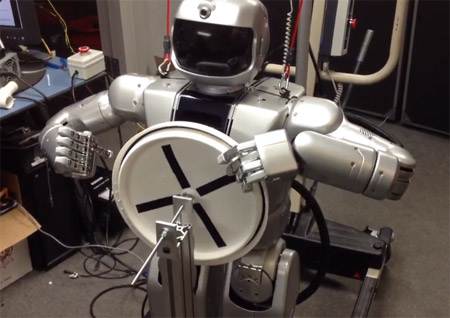
\includegraphics[width=1.0\columnwidth]{./pix/hubo_valve.png}
  \caption{Daniel M. Lofaro (Left) using Hubo-Ach on Hubo (Right) to turn a valve at Drexel University.  
The valve turing is being developed in conjunction with Dmitry Berenson at WPI for the DARPA Robot Challenge with the Track-A team DRC-Hubo.
The video of the valve turning example can be found at http://drc-hubo/video/valve-example/.}
  \label{fig:valve}
\end{figure}

Fig.~\ref{fig:graph} shows an example of the Hubo-Ach system in action.
This exampe shows how Hubo-Ach was used to create a closed loop system that includes the use of ROS.
\textit{Process 1} is the Hubo-Ach daemon.
The daemon is comunicating with the Hubo robot via the CAN bus and updating the state data with a period of 5 $ms$.
The state data is published to the \textbf{Feedback} Ach Channel at this rate.
\textit{Process 2} is the feedforward portion of the Hubo-Ach to ROS and ROS to Hubo-Ach bridge.
It reads the \textit{Feedback} channel at given rate and publishes the data to the ROS topic \textit{\textbf{Feedback}}.  
The data published is the state data found in \textbf{Feedback} at the time it was read.
The rate it is read at can be the same or different from that of \textit{Process 1} and does not have to be regular.
\textit{Process 2} is a Hubo visulizer that reads the state data off of the ROS topic \textit{\textbf{Feedback}} and applies it to the OpenHUBO model in rviz.
\textit{Process 3} is the closed loop controler.  
It takes in the state data from the \textit{\textbf{Feedback}} ROS topic, performs a control such as visual servoing, impeedence control, pathplanning etc.
The resulting joint space references are published to the \textit{\textbf{Feedforward}} ROS topic.
\textit{Process 4} is event based where when a new message is posted on \textit{\textbf{Feedforward}} the second part of the Hubo-Ach to ROS and ROS to Hubo-Ach bridge it posts the references in the ROS message to the \textbf{Ref} Ach Channel.
To allow step inputs to be commanded to the robot without damaging the joints a lowpass filter is added between ROS and the Hubo-Ach daemon \textit{Process 5}.  
This filter reduces the \textit{jerk} on each joint.
The resulting filtered reference is posted to the \textbf{Feedforward} Ach channel where the Hubo-Ach daemon can read it and command the Hubo.

Hubo-Ach has been used in numerous projects by multiple research labs.  
As of December 2012 this includes labs at MIT, WPI, Ohio State, Purdue, Georgia Tech, and Drexel University.
These projects primarally revolve around development for the DARPA Robot Challenge\footnote{DARPA Robot Challenge: http://www.theroboticschallenge.org/} team DRC-Hubo\footnote{DRC-Hubo Homepage: http://drc-hubo.com/} lead by the Drexel Autonomous Systems Lab at Drexel University.
The projects include rough terrain walking, ladder climbing, valve turing, vehicle ingress/egress and more.
Fig.~\ref{fig:valve} shows the Hubo using the Hubo-Ach system to turn a valve.
The video of the valve turning example can be found at http://drc-hubo/video/valve-example/. 

The key point is that Hubo-Ach updates the state data in the \textbf{Feedback} channel and commands the motors with the references set in the \textbf{Feedforward} channel in real-time.  
The system is inherently robust because the controllers are run in seperate processes.
The failed process can then be restarted with no harm done to the robot.
In addition the controlelrs can run at killohertz rates becuse they comunicate with the Hubo-Ach daemon via the high-speed low-latancy IPC Ach.
Hubo-Ach is legerages ubicquidous robot interface software such as ROS and MATLAB which inherently increases the capiability of the system.
It was written entirelly in C allowing easy intergration with existing software.
Hubo-Ach is a tested and functional creating an easy to use interface between the electro-mechanical and control algorithms of complex system Hubo the full-size humanoid robot.
